\chapter{Magnetic Inversion}\label{Chp:cook:magnetic inversion}
This gives an intro to standard magnetic inversion


\begin{itemize}
\item All onshore station points are above mean see level with positive
elevation.

\item Data have to be gridded to a rectangular in latitude and longitude
for gravity station records.

\item All corrections was applied for observed gravity data including
tidal, latitude and elevation. Bouguer anomalies have been utilized as
gravity data which was calculated using a density of $2.67 \frac{t}{m^3}$.

\item In this stage of processing, data have to contain positive and
negative numbers for Bouguer anomaly.
\end{itemize}

\section{Magnetic Data} 

Although Magnetic and gravity methods are almost the same, Magnetic has its own complexity, elaboration and instability and it is very localized. Outer core of the Earth has a convection current which produce a magnetic field through the earth. Magnetic fields are not central and their directions vary with azimuth. Its north pole is in the south of the Earth and south pole is in north of the earth. Meantime magnetic poles and its axis are not exactly coinciding with geographical one. The lines of magnetic field come out from south magnetic pole and go into north magnetic field. Also poles are shifted continuously.

The basic magnetic field or magnetic flux density in any medium is $B$. Meanwhile $H$ is a parameter proportional to $B$ in non magnetizable material. In magnetizable material $H$ is describe how $B$ is changed with polarization or magnetization.

All material magnetic behavior, refer on magnetic moments of atoms or its ions, have a character. The ability of material to be magnetized in an external magnetic field, introduces as magnetic susceptibility. Based on their magnetic susceptibility, material is compartmented in three main classes: diamagnetism, paramagnetism and ferromagnetism.

Increasing magnetic field anomalies over subsurface geological structure illustrate contrast between magnetization in neighboring rock properties.

Some particular ions in atmosphere release electrical currents so this external magnetic field acquire in the surface of the magnetic observation. Also in day time sun heating cause more motion in these particle. This time related changes of magnetic field are the diurnal variation which depends on the latitude of observation point. 

Magnetic field intensity differs in latitude, longitude and altitude. The vertical gradient of magnetic field gives the elevation correction. It is varied from magnetic equator to magnetic poles which is generally small. Latitude correction is zero in magnetic poles and equator and reaches a maximum at intermediate latitude.

The shape of the magnetic anomaly is distinguished with the form and the depth of the structure and depends on magnetization contrast and the objects orientation in the earth.

International Geomagnetic Reference Field (IGRF) is a mathematical description of Global magnetic field and it  is provided each 5 year.

In comparison to the correction of gravity observation, magnetic survey needs very few corrections. after compensation of diurnal effect, latitude and elevation corrections are applied. Then global magnetic field should be subtracted from data. finally magnetic anomaly is used in geophysical processing.

\begin{figure}
\centering
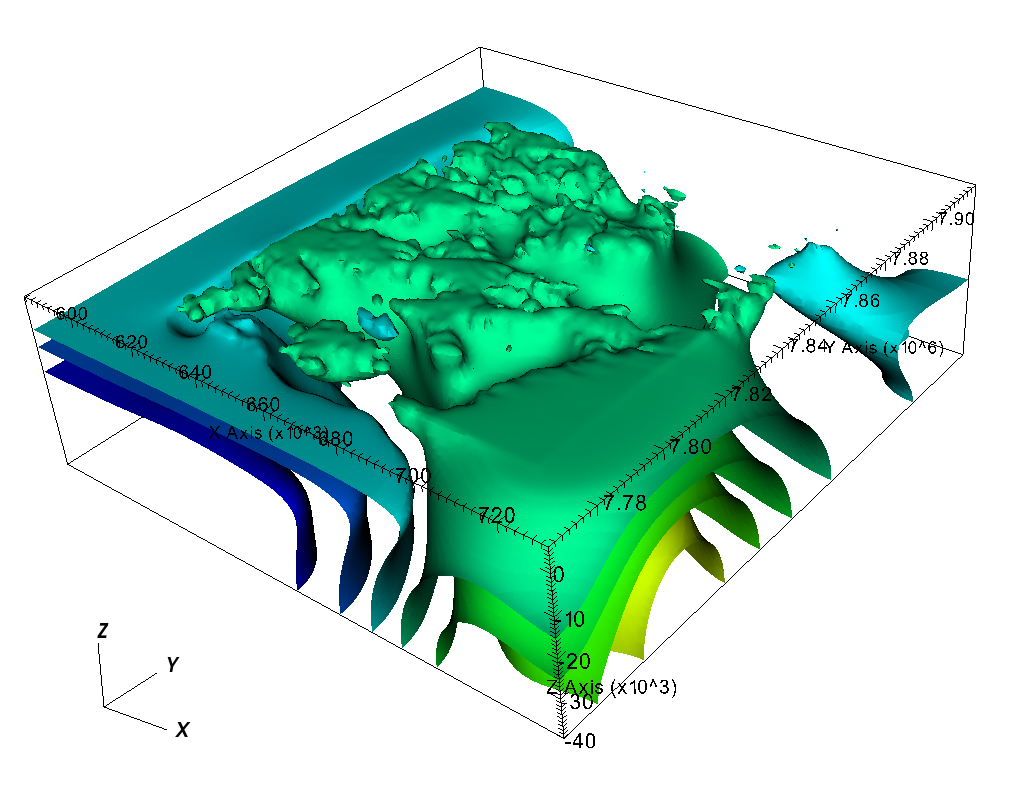
\includegraphics[width=\textwidth]{sus3Dc.png}
\caption{Contour image through a 3 dimensional magnetic inversion which presents discrepancy in susceptibility. The magnetic of padding area of the model is not defined. Increasing and decreasing in susceptibility are indicated with red color and blue color respectively.}
\end{figure}

\begin{figure}
\centering
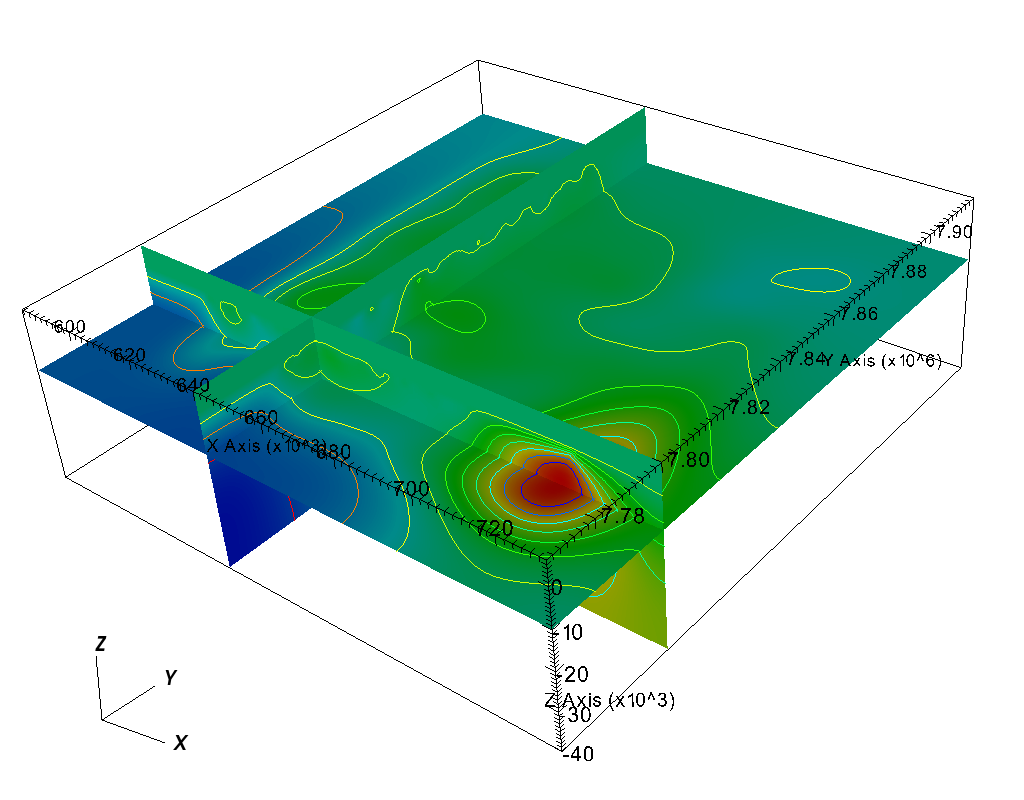
\includegraphics[width=\textwidth]{sus3D.png}
\caption{Depth image across previous 3D magnetic inversion which presents discrepancy in susceptibility. Diversity in susceptibility are detected with colors and contours.}
\end{figure}

\section{Input File} 

This module of magnetic inversion needs two input files which contain magnetic anomalies and some constraint factors. The firs file include magnetic anomalies, in which all corrections were applied previously, and the location (latitude and longitude) and elevation of the observed place are defined precisely.

The next file which consists some factors to figure the inversion escripts. Again in magnetic inversion, a padding area present around the real data to smooth the effects of cutting data in boundaries.
 
A small part of sample of run_mag2D:

\begin{verbatim}
mu=10
THICKNESS=20.*U.km
DATASET='NSW_east.nc'
PAD_X = 0.2
PAD_Y = 0.2
l_air = 6. * U.km
n_cells_v = 25
\end{verbatim}

Almost all of constraints factors are the same as gravity instead of Mu factor.\\

\begin{description} 	

\item[mu]
It is defined in accordance with the noise of data and it has a wide range to select from 0.0001 to 100. Also its does not have same value for 2D and 3D inversion.

\end{description}

\section{Output File}

After inversion completion, an output file with silo extension is created which is consisted inversion result. this file show the input data as magnetic anomaly and inverted susceptibility separately. The objective is indeed to  predict a susceptibility model with have a best fit with input data. the inversion go forward to attain an acceptable volume for error in its mathematical function. 


\section{Reference}

As some examples there are several inversions which have ran in some synthetic magnetic data sets . Here comparisons between synthetic susceptibility and inverted one are shown.

Some of the presumptions are the same for all of the examples to simplify the situation to make a logical comparison between synthetic input and output. which is as followed:

\begin{verbatim}
depth_offset=0.*U.km
l_data = 100 * U.km
l_pad=40*U.km
THICKNESS=20.*U.km
l_air=6*U.km
\end{verbatim}

The others assumptions comes with each example.

\begin{enumerate}
\item A 2D magnetic susceptibility area is created with one maximum and one minimum in two sides. that after inversion the main boundary of our dataset  have got a best simulation.(\ref{fig:mag2D2}) 
\begin{verbatim}
n_cells_in_data=100
n_humbs_h= 2
n_humbs_v=1
mu=1.
\end{verbatim}

\begin{figure}
\centering
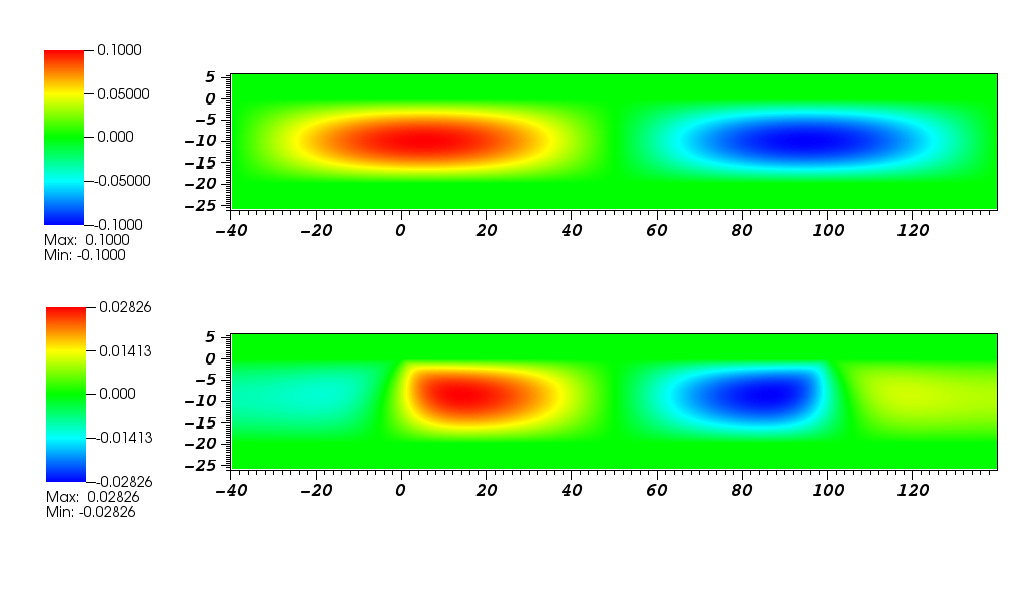
\includegraphics[width=\textwidth]{mag2D2.png}
\caption{2D magnetic inversion up) the reference model  down)the inverted model}
\label{fig:mag2D2}
\end{figure}

\item A 2D magnetic area with two maximum and two minimum intermittent is suggested. In this initial model two of the humps are located in the padding area which is not important after inversion, is omitted then. so in the result just two humps in middle of the boundary is observable.(\ref{fig:mag2D4})

\begin{verbatim}
n_cells_in_data=100
n_humbs_h= 4
n_humbs_v=1
mu=1.
\end{verbatim}

\begin{figure}
\centering
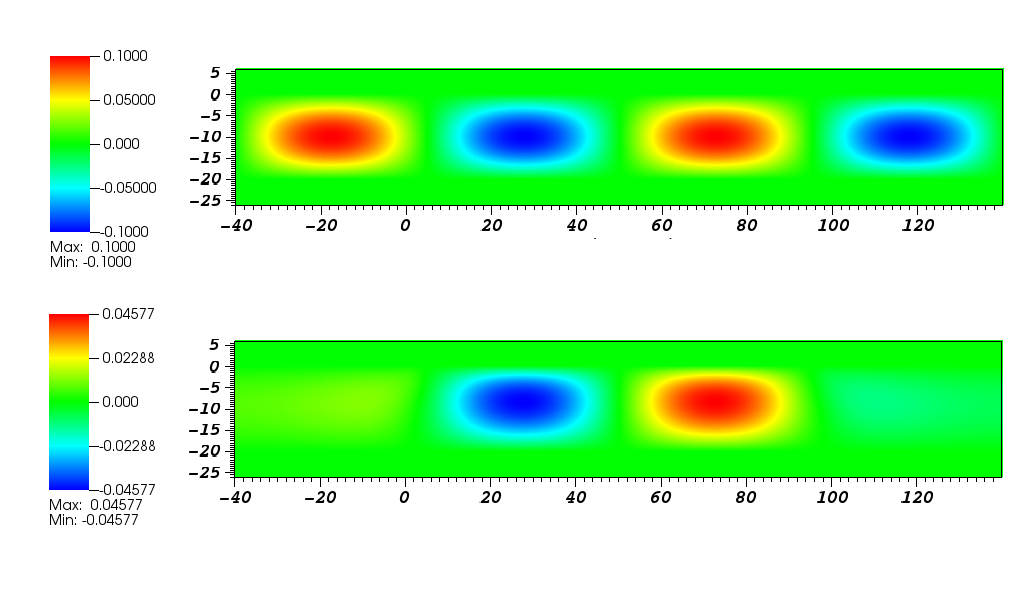
\includegraphics[width=\textwidth]{mag2D4.png}
\caption{2D magnetic model up) the reference model  down)the inverted model}
\label{fig:mag2D4}
\end{figure}

\item A 3D magnetic model with one humbs in the middle of the area is proposed that surrounded all main and padding. after inversion just the main area is objective which have a good result for inversion.(\ref{fig:mag3D1-ref} and \ref{fig:mag3D1})

\begin{verbatim}
n_humbs_h=4
n_humbs_v=1
mu=0.0001
n_cells_in_data=50
\end{verbatim}

\begin{figure}
\centering
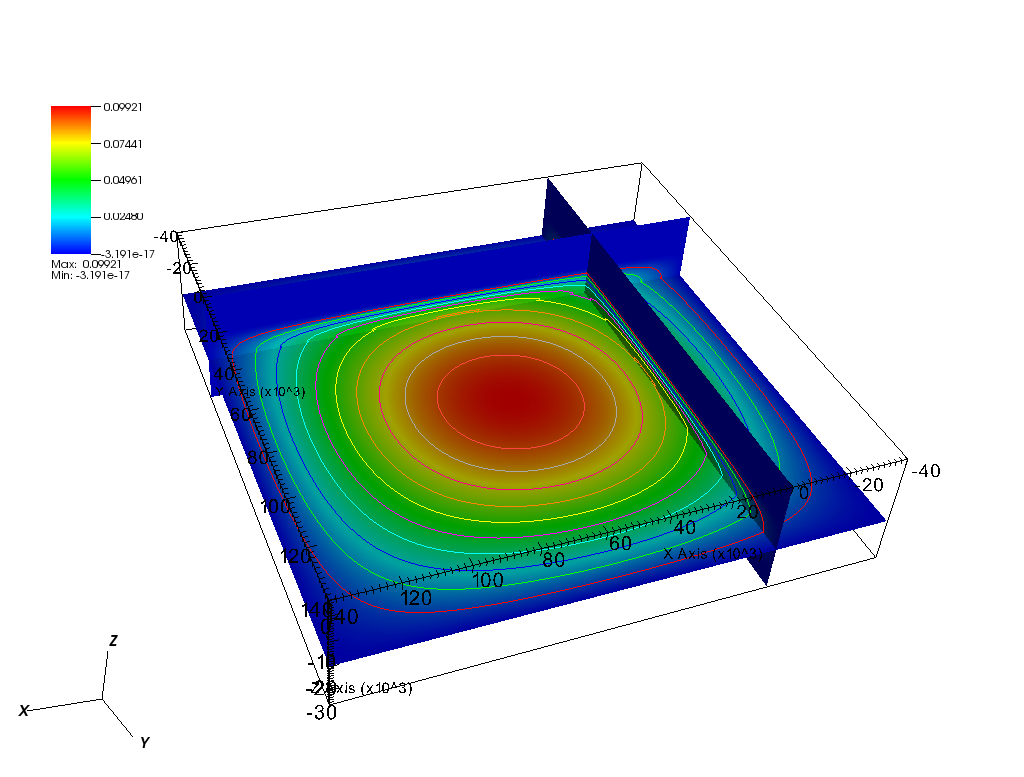
\includegraphics[width=\textwidth]{mag3D1-ref.png}
\caption{3D magnetic reference model with one maximum susceptibility}
\label{fig:mag3D1-ref}
\end{figure}

\begin{figure}
\centering
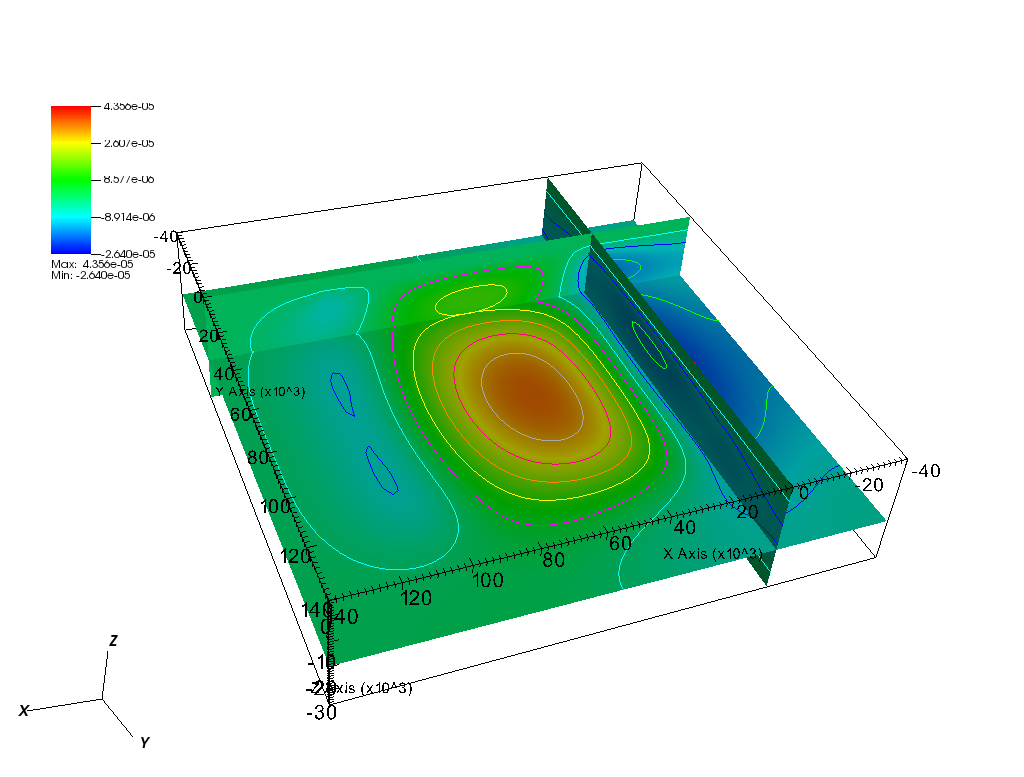
\includegraphics[width=\textwidth]{mag3D1.png}
\caption{3D magnetic inversion result}
\label{fig:mag3D1}
\end{figure}
\end{enumerate}
